\chapter{Results}
\label{results}
For the evaluation both the balanced and the unbalanced version were compiled using my Clang and GNU cross compiler toolchain.
Both versions were compiled using the \texttt{-O0} option, to avoid the influence of any optimizations.
\Cref{tbl:properties} shows a summary of the properties of both versions.
\Cref{fig:rc4,fig:aes} contain histograms of \hammingw{}s during execution of the balanced and unbalanced code.
A more detailed discussion of the results follows.
  
\begin{table}[h]
  \begin{tabular}{|l|l|l|l|l|}
    \hline
    & \multicolumn{2}{c|}{RC4}  & \multicolumn{2}{c|}{AES} \\
    \cline{2-5}
    & unbalanced & balanced & unbalanced & balanced \\
    \cline{2-5}
    Balancedness      & 0.236 & 0.455 & 0.362  & 0.584 \\
    No. of Operations & 77349 & 401287 & 83549 & 2396186 \\
    Relative Increase & 1 & 5.19 & 1 & 26.68 \\
    Code Size            & 3.5 KB & 3.1 KB & 5.8 KB & 14 KB \\
    \hline
  \end{tabular}
  \caption{Properties of balanced and unbalanced test code}
  \label{tbl:properties}
\end{table}

\begin{figure}[hp]
  \centering
  \begin{subfigure}[b]{0.49\textwidth}
    \begin{tikzpicture}
\begin{axis}[
    ybar,
    bar width=0.015\textwidth,
    enlargelimits=0.05,
    xtick={0,8,16,24,32},
    width=\textwidth,
]
\addplot[pantone289,fill=pantone289!40] table [x=i, y=unbalanced-total, col sep=comma] {data/rc4.csv};
\end{axis}
\end{tikzpicture}

    \caption{Unbalanced RC4}
  \end{subfigure}
  \begin{subfigure}[b]{0.49\textwidth}
    % This file was created by matplotlib2tikz v0.7.4.
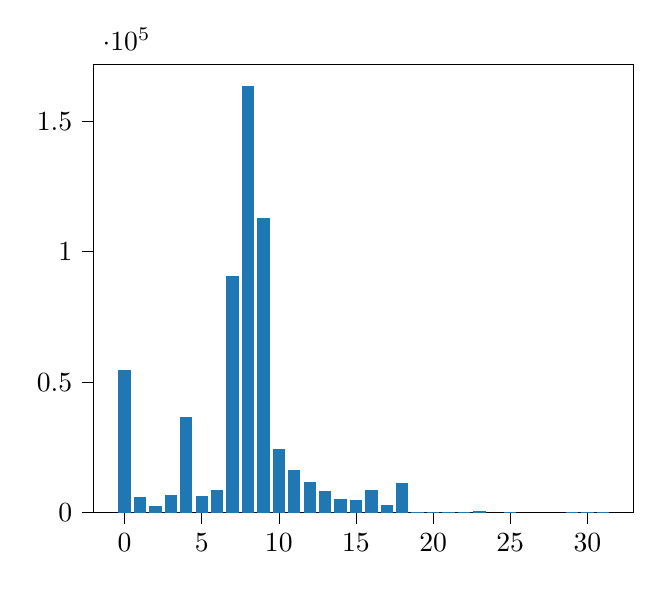
\begin{tikzpicture}

\definecolor{color0}{rgb}{0.12156862745098,0.466666666666667,0.705882352941177}

\begin{axis}[
tick align=outside,
tick pos=left,
x grid style={white!69.01960784313725!black},
xmin=-1.99, xmax=32.99,
xtick style={color=black},
y grid style={white!69.01960784313725!black},
ymin=0, ymax=171938.55,
ytick style={color=black}
]
\draw[fill=color0,draw opacity=0] (axis cs:-0.4,0) rectangle (axis cs:0.4,54571);
\draw[fill=color0,draw opacity=0] (axis cs:0.6,0) rectangle (axis cs:1.4,6050);
\draw[fill=color0,draw opacity=0] (axis cs:1.6,0) rectangle (axis cs:2.4,2313);
\draw[fill=color0,draw opacity=0] (axis cs:2.6,0) rectangle (axis cs:3.4,6824);
\draw[fill=color0,draw opacity=0] (axis cs:3.6,0) rectangle (axis cs:4.4,36773);
\draw[fill=color0,draw opacity=0] (axis cs:4.6,0) rectangle (axis cs:5.4,6353);
\draw[fill=color0,draw opacity=0] (axis cs:5.6,0) rectangle (axis cs:6.4,8761);
\draw[fill=color0,draw opacity=0] (axis cs:6.6,0) rectangle (axis cs:7.4,90865);
\draw[fill=color0,draw opacity=0] (axis cs:7.6,0) rectangle (axis cs:8.4,163751);
\draw[fill=color0,draw opacity=0] (axis cs:8.6,0) rectangle (axis cs:9.4,112999);
\draw[fill=color0,draw opacity=0] (axis cs:9.6,0) rectangle (axis cs:10.4,24463);
\draw[fill=color0,draw opacity=0] (axis cs:10.6,0) rectangle (axis cs:11.4,16480);
\draw[fill=color0,draw opacity=0] (axis cs:11.6,0) rectangle (axis cs:12.4,11631);
\draw[fill=color0,draw opacity=0] (axis cs:12.6,0) rectangle (axis cs:13.4,8125);
\draw[fill=color0,draw opacity=0] (axis cs:13.6,0) rectangle (axis cs:14.4,5158);
\draw[fill=color0,draw opacity=0] (axis cs:14.6,0) rectangle (axis cs:15.4,4929);
\draw[fill=color0,draw opacity=0] (axis cs:15.6,0) rectangle (axis cs:16.4,8458);
\draw[fill=color0,draw opacity=0] (axis cs:16.6,0) rectangle (axis cs:17.4,2812);
\draw[fill=color0,draw opacity=0] (axis cs:17.6,0) rectangle (axis cs:18.4,11488);
\draw[fill=color0,draw opacity=0] (axis cs:18.6,0) rectangle (axis cs:19.4,374);
\draw[fill=color0,draw opacity=0] (axis cs:19.6,0) rectangle (axis cs:20.4,342);
\draw[fill=color0,draw opacity=0] (axis cs:20.6,0) rectangle (axis cs:21.4,206);
\draw[fill=color0,draw opacity=0] (axis cs:21.6,0) rectangle (axis cs:22.4,170);
\draw[fill=color0,draw opacity=0] (axis cs:22.6,0) rectangle (axis cs:23.4,456);
\draw[fill=color0,draw opacity=0] (axis cs:23.6,0) rectangle (axis cs:24.4,0);
\draw[fill=color0,draw opacity=0] (axis cs:24.6,0) rectangle (axis cs:25.4,179);
\draw[fill=color0,draw opacity=0] (axis cs:25.6,0) rectangle (axis cs:26.4,0);
\draw[fill=color0,draw opacity=0] (axis cs:26.6,0) rectangle (axis cs:27.4,0);
\draw[fill=color0,draw opacity=0] (axis cs:27.6,0) rectangle (axis cs:28.4,2);
\draw[fill=color0,draw opacity=0] (axis cs:28.6,0) rectangle (axis cs:29.4,8);
\draw[fill=color0,draw opacity=0] (axis cs:29.6,0) rectangle (axis cs:30.4,41);
\draw[fill=color0,draw opacity=0] (axis cs:30.6,0) rectangle (axis cs:31.4,16);
\end{axis}

\end{tikzpicture}

    \caption{Balanced RC4}
  \end{subfigure}

  \begin{subfigure}[b]{\textwidth}
    % This file was created by matplotlib2tikz v0.7.4.
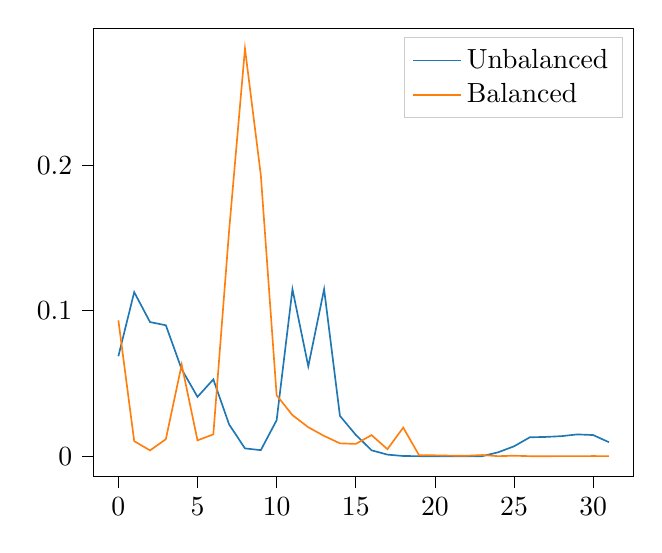
\begin{tikzpicture}

\definecolor{color0}{rgb}{0.12156862745098,0.466666666666667,0.705882352941177}
\definecolor{color1}{rgb}{1,0.498039215686275,0.0549019607843137}

\begin{axis}[
legend cell align={left},
legend style={draw=white!80.0!black},
tick align=outside,
tick pos=left,
x grid style={white!69.01960784313725!black},
xmin=-1.55, xmax=32.55,
xtick style={color=black},
y grid style={white!69.01960784313725!black},
ymin=-0.0140054362142874, ymax=0.294114160500036,
ytick style={color=black}
]
\addplot [semithick, color0]
table {%
0 0.0686886708296164
1 0.112735781975203
2 0.0921666731308743
3 0.0899559141036083
4 0.0597292789822751
5 0.0407632936430982
6 0.0527737915163738
7 0.0217455946424647
8 0.0053394355453852
9 0.00412416450115709
10 0.0247062017608502
11 0.114713829525915
12 0.0617719686098075
13 0.114752614772007
14 0.0276926657099639
15 0.014647894607558
16 0.00403366559360819
17 0.00106013005985856
18 0.000116355738277159
19 0
20 0
21 0
22 0
23 0
24 0.00268911039573879
25 0.0067744896508035
26 0.0129801290255853
27 0.0132257689175038
28 0.0137558339474331
29 0.014958176576297
30 0.0145186104539167
31 0.00957995578481946
};
\addlegendentry{Unbalanced}
\addplot [semithick, color1]
table {%
0 0.0933479074509321
1 0.0103489919568661
2 0.00395656502417046
3 0.0116729786964718
4 0.0629030547487333
5 0.0108672968433009
6 0.0149863666998519
7 0.155431595729031
8 0.280108724285749
9 0.193293511096514
10 0.041845849626581
11 0.0281903119750666
12 0.0198957232149272
13 0.0138984396114937
14 0.00882315710967195
15 0.00843143493477569
16 0.0144680618134171
17 0.00481014303846404
18 0.0196511106777649
19 0.000639755866424449
20 0.000585017396569951
21 0.000352378899688333
22 0.000290798121102022
23 0.000780023195426601
24 0
25 0.0003061933157486
26 0
27 0
28 3.42115436590614e-06
29 1.36846174636246e-05
30 7.0133664501076e-05
31 2.73692349272492e-05
};
\addlegendentry{Balanced}
\end{axis}

\end{tikzpicture}
    \caption{Scaled Hamming weight histograms for RC4}
  \end{subfigure}
  \caption{Hamming weight histograms for balanced and unbalanced RC4}
  \label{fig:rc4}
\end{figure}

\begin{figure}[hp]
  \centering
  \begin{subfigure}[b]{0.49\textwidth}
    \begin{tikzpicture}
\begin{axis}[
    ybar,
    bar width=0.015\textwidth,
    enlargelimits=0.05,
    xtick={0,8,16,24,32},
    width=\textwidth,
]
\addplot[pantone289,fill=pantone289!40] table [x=i, y=unbalanced-total, col sep=comma] {data/aes.csv};
\end{axis}
\end{tikzpicture}

    \caption{Unbalanced AES}
  \end{subfigure}
  \begin{subfigure}[b]{0.49\textwidth}
    \begin{tikzpicture}
\begin{axis}[
    ybar,
    bar width=0.015\textwidth,
    enlargelimits=0.05,
    xtick={0,8,16,24,32},
    width=\textwidth,
    xlabel={\hammingw{}},
    ylabel={Occurences}
]
\addplot[pantone289,fill=pantone289!40] table [x=i, y=balanced-total, col sep=comma] {data/aes.csv};
\end{axis}
\end{tikzpicture}

    \caption{Balanced AES}
    \label{fig:aes-balanced}
  \end{subfigure}

  \begin{subfigure}[b]{\textwidth}
    \begin{tikzpicture}
\begin{axis}[
    ybar=2*\pgflinewidth,
    bar width=0.00725\textwidth,
    enlargelimits=0.05,
    xtick={0,8,16,24,32},
    width=\textwidth
]
\addplot[pantone289,fill=pantone289!40] table [x=i, y=unbalanced-scaled, col sep=comma] {data/aes.csv};
\addplot[pantone144,fill=pantone144!40] table [x=i, y=balanced-scaled, col sep=comma] {data/aes.csv};
\end{axis}
\end{tikzpicture}

    \caption{Scaled Hamming weight histograms for AES}
    \label{fig:aes-comp}
  \end{subfigure}
  \caption{Hamming weight histograms for balanced and unbalanced AES}
  \label{fig:aes}
\end{figure}

\section{Robustness}
As visible in both \Cref{fig:rc4} and \Cref{fig:aes}, the balanced version has a much narrower distribution of \hammingw{}s.
Although my balancing does not reach the perfect outcome of identical \hammingw{}s for all operations, it shows a significant move towards it.
Perfect balancing cannot be reached with current ALUs, as their design forces imbalances in intermediate values.
For this reason the balancedness in \Cref{tbl:properties} is the ratio of \hammingw{}s in the range between 7 and 9, and not only the ratio of \hammingw{}s of 8.

The balancedness metric in \Cref{tbl:properties} is a very simplistic metric, however, and the histograms in \Cref{fig:rc4,fig:aes} paint a much clearer picture of the effectiveness of my balanced arithmetic.
The balancing works especially well for AES, as shown in \Cref{fig:aes-balanced}.
A large number of values is perfectly balanced, as signified by the large value at 8.
This is due to the large number of table lookups.
In the beginning of my code the lookup tables are copied onto the stack, which causes them to be balanced.
Another cause is the frequent usage of XOR operations, which are perfectly balanced in my arithmetic.
The additional spike around 9 is likely caused by the large number of loops in AES, causing a many increment operations and therefore additions.
However, I am not entirely certain this is the only reason, as RC4, which has a similarly high ratio of increments, does not exhibit the same behavior.

For RC4 the balancing does not work as well.
The largest spike in \hammingw{}s is at 7 here, and the variance is higher.
This value is only an intermediate \hammingw{} for balanced subtraction, which does not occur in RC4.
Due to this I assume this is caused by array accesses, which require the value to be unbalanced before it can be used as index.
Another possibility is that this is some artifact not directly linked to my arithmetic.
The number of values with \hammingw{} 7 is roughly the same as in AES, which supports this theory.

For both AES and RC4 the histograms indicate increased robustness, and the reduced variance in histograms should reduce the amount of information retrievable by an attacker.

\section{Performance}
Unfortunately the performance impact of my balancing pass is rather large.
As shown in \Cref{tbl:properties} the number of operations increases by a factor of 5.19 for RC4, and by a factor of 26.68 for AES.
A possible reason for this discrepancy is the larger number of array accesses in AES, which all require unbalancing.

Code size does not increase as drastically.
For RC4, the balanced code actually requires \emph{less} memory than the unbalanced version.
This might be caused by a simple dead code removal routine I added to reduce the lines of code in the \ir{} files during debugging.
The code size for balanced AES should also be fine for most embedded platforms, as that already includes all lookup tables.
The moderate increase in code size is caused by the balanced operators being implemented as functions, and not being inlined during compilation.
Adding inlining for the operators would allow for an additional memory-performance tradeoff, if desired.
Calling the operator functions causes overhead (storing and restoring of registers, etc.), which is likely the main cause of the increased memory size.
Another probable cause is the unbalancing instructions before array indexing.
These are also implemented as functions, again causing overhead.

The code was not optimized (compiled with \texttt{-O0}), so there was no loop unrolling.
This would cause an additional increase in code size for the case of inlined operators.

While the performance impact is (prohibitively) large, please note that performance was not a focus for my thesis.
